\chapter{Software Design and Implementation}
\label{chap:software-design}
 
\section{Background}
This section will provide details of the existing software and services that are leveraged to create the Collaborative Environment. For each, we provide the reasoning for its use as well as a technical description.

\subsection{Symfony}
The Collaborative Environment is built using Symfony Standard Edition, an open-source, object-oriented PHP framework designed around the Model-View-Controller (MVC) software architecture. Using Symfony to create the Collaborative Environment encourages the use of design patterns that are well understood and allows for more of the development time to focus on application features rather than reimplementing standard components of web applications.

The MVC architecture separates an application's business logic, that is, all of the algorithms which process the exchange of data between an interface and a database, from its user interfaces. The \emph{model} consists of object representations of application data (Entities) and a persistence layer, which will store and retrieve entities via a databases management system. The \emph{view} will render a model object into a user interface, such as a web page. The \emph{controller} is what mediates transactions between the user and the application. The typical control flow of a basic MVC application is:

\begin{singlespacing}
\begin{enumerate}
	\item Client makes a request
	\item Controller receives the request and transforms it into a manipulation of the Model
	\item The updated Model is saved to the database by the persistence layer from the Controller
	\item A View is generated by the Controller which makes the changes to the Model visible
	\item The Controller responds to the Client's request with the generated View.
\end{enumerate}
\end{singlespacing}

Symfony Standard Edition comes with many software bundles which extend the core Symfony framework to provide an enterprise-grade application skeleton. Three of the key bundles included are the Security, Doctrine, and Twig bundles, which provide user-rights management, an object-relational mapper, and a template engine respectively.

\subsubsection{Security}
Security in Symfony is handled by a two-step process: authentication and authorization. The authentication step identifies a user and is typically accomplished by having a user first visit the website, at which point they are authenticated as an anonymous user, and then having them provide a set of credentials to authenticate them as a specific user. Authorization occurs when a user attempts to access a resource of an application. Symfony allows for a set of user roles to be defined, of which each user has a set of, as well as an access control list, to determine exactly what resources any given user has access to.

Controllers are aware of what the current user's authentication is and, as such, can be configured to only allow processing to occur if and only if the current user has a given role. While an Entity will generically describe all instances of a piece of data in an application, if the currently authenticated user should only have access to an exact instance of an entity, an entry can be added to an access control list for that particular user-entity instance pair.

These features provide the Collaborative Environment with a powerful and robust mechanism that is essential to securing the Student data being tracked.

\subsubsection{Doctrine}
In a dynamic web application, Entities are constantly being created, read, update, and deleted. To keep track of these changes, it is natural to consider using a database management system (DBMS) such as MySQL or PostgreSQL. In an object-oriented program, these Entities often contain non-scalar data (e.g. lists, arrays) that must be persisted by a DBMS, which can be problematic because a DBMS can often only store scalar data (e.g. strings, integers). Using an object-relational mapper (ORM), such as Doctrine, solves this problem by managing the transformation to and from scalars/non-scalars when persisting an object.

As an example of how an ORM operates, let's consider an object-oriented system where a Student is enrolled in a set of Courses. Naturally, we would have two Entity objects, Student and Course. The fields of the Student entity could be an ID, a name, and a list of Courses that they're enrolled in (consider this to be a many-to-many relationship). The fields of the Course Entity could be a name and number. When a new Student has been created and they are enrolled in, perhaps, two different Courses and the ORM is told to persist this data, it will store the scalar data in the  DBMS as its native types (names map to varchar, IDs and numbers map to integer), but for the Student's list of enrolled courses, since we established that there is a many-to-many relationship, the ORM will manage a Student ID-Course number tuple (Student 1 is enrolled in Course 1, Student 1 is enrolled in Course 2). Of course, when this data is requested from the DBMS, the ORM will convert the data back into Entity objects.

\subsubsection{Twig}
When a Controller has to return a new response, it is common for the View to be defined as a template that will be rendered though an engine, such as Twig, rather than explicitly crafted in the desired output format. For example, this could be accomplished by designing a Twig template that will output specific Model Entity variables and have it be processed into HTML by the Twig engine instead of just writing a mixture of HTML and PHP directly.

There are many benefits to using a template engine, such as:

\begin{description}
	\item [Template inheritance] Defining a parent or a layout template that can be inherited from children allowing for a consistent theme across an application.
	\item [Syntax] Provides numerous shortcuts for applying common patterns to variables such as escaping output and modifying control flow.
	\item [Speed] After compiling a template, the result will be optimized and low-overhead PHP when compared to freehand coding.
\end{description}

\subsection{Khan Academy}
The Khan Academy is a nonprofit organization that aims to better global education by providing free, high-quality resources to anyone anywhere. \cite{khan-website-about} On their website, they provide in excess of 2700 videos that teach varying topics in STEM fields. The organization has been provided with the financial support and public accolades of large entities such as The Bill \& Melinda Gates Foundation and Google \cite{khan-wiki-sources} indicating that they produce noteworthy content. The videos that Khan Academy hosts are all created by Salman Khan who holds an MBA from Harvard and three science degrees from MIT. Each is produced in a fairly consistent manner using a software whiteboard, a screen capture program, and a microphone while typically lasting about 10 minutes.

As stated in \S \ref{sec:overview-goals} and \S \ref{sec:overview-features}, students using the Collaborative Environment should have access to supplemental learning resources and will have the ability to take quizzes given by their teachers and teaching assistants. The Khan Academy videos are ideal for this use as they are concise and short enough to be associated with individual quizzes that are created in the Collaborative Environment. If a student, while taking a quiz, feels that they are in need of some assistance, a link to the an appropriate Khan Academy video will be readily available to them.

\section{Features}
\label{sec:design-features}
We now describe the main features of the Collaborative Environment as previously outlined in \S \ref{sec:overview-features}. Each subsection henceforth provides the concept, design, and implementation of an individual feature. They have been arranged in such a way that each successive feature will build on the previously introduced ones.

%%%% Academic
\subsection{Academic Year}
\label{subsec:design-year}
In a traditional document-based teaching environment, student data is stored in numerous grade books  or spreadsheets which are held by many different people in many different places. Each teacher, for instance, would have their own set of student records and a district will have a permanent record for each student containing information such as their standardized test scores. If an administrator managed to collect all of this data into a single place, however frustrating that may be, the next thing they would have to do to it, before any type of analysis, would be to group it all by what year the record corresponds to.

As the Collaborative Environment will be collecting data year after year, an Academic Year entity is required. Teachers, Teaching Assistants, and Students all have data associated with them that can change on an annual basis. Students will be taking different classes, have taken different standardized tests, and participated in different activities as well as be in a different grade altogether or have graduated. Each year can also bring with it a different round of quizzes and surveys and even new Teachers or Teaching Assistants.


\subsubsection{Design}
The Year entity is really very simple, just a primary key identifier, \emph{id}, and the year itself as an integer, \emph{year}. Explicitly storing the years that the Collaborative Environment will be tracking in a table allows consistency throughout the entire application and customization by an administrator. An alternative implicit design would have been to keep a \emph{date} column in each entity that was going to have time-sensitive content added to it and the server would be responsible for getting the current year from the operating system, but problems arise if the system's time and date are not correct. 

\begin{figure}[h!]
	\centering
	\fbox {
		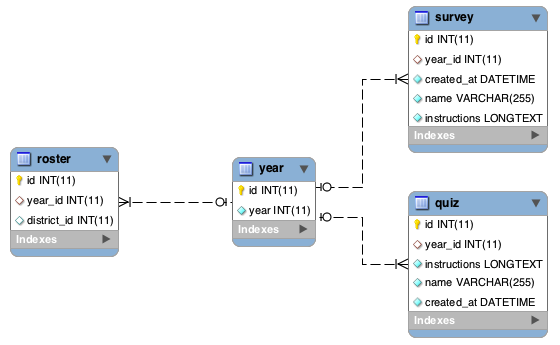
\includegraphics[width=0.7\textwidth]{figures/er/year}
	}
	\caption{Year Enhanced Entity-Relationship (EER) Diagram}
	\label{fig:er-year}
\end{figure}

We see in Figure \ref{fig:er-year}, that the year entity appropriately maintains a one-to-many relationship with each of the tables that reference it. In an EER diagram such as this, each box represents a table in a database and each row in a box corresponds to a column in that table. A connecting line indicates that a relationships exists between its connected tables. If we take the relationship between the year and survey tables as an example, the line, which is drawn using Crow's Foot notation, indicates that a survey can be given during one year and that a year can have many surveys given during it. This diagram additionally indicates that many quizzes (see \S \ref{subsec:design-quiz}) and many rosters (see \S \ref{subsec:design-district}) can also only be associated with only one year.

The user's choice of which year they want to have as their current context for data viewing and manipulation will have to persist between each page of the Collaborative Environment. Having to constantly select what year to interact . Therefore, once a user initially visits the web site, a PHP session variable will be established that tracks the year they select which will then be used by subsequent SQL queries to retrieve the requested data.

\subsubsection{Implementation}
As established in the previous section, the selected year must be persisted from page-to-page as well as be accessible in such a way that it will not require a user to constantly have to interact with a selector.

This was implemented by having a year selector list appear in the upper-right corner of each page in the Collaborate Environment, as shown in Figure \ref{fig:screens-year}. The list is populated by making an asynchronous HTTP GET request to the URL \texttt{/year} which will both provide all available academic years that have been configured and indicate which is the current year as selected by the user.

\begin{figure}[h!]
	\centering
	\fbox{
		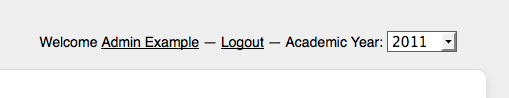
\includegraphics[width=0.6\textwidth]{figures/screens/year/year}
	}
	\caption{Year Selector Highlight}
	\label{fig:screens-year}
\end{figure}

Upon choosing a year from the selection, if it differs from the currently selected year, then an HTTP POST request will be sent to \texttt{/year/change/\textit{selected-year}}. This will cause the year PHP session variable to be updated to \emph{selected-year}. If the server responds with a success message, then the current web page will be refreshed and any changes to the data that are dependent on the year will be reflected.

%%%% Users
\subsection{User Management}
\label{subsec:design-user}
A User entity is perhaps the most fundamental object in the Collaborative Environment.  Users of each class, as defined in \S \ref{sec:overview-user-classes}, with the exception of anonymous, will be required to have an account with this system, and that account is what the User entity represents. The set of users minus anonymous will be referred to as ``registered users''.

	This entity facilitates the fulfillment of the Collaborative Environment's goal of logging user data by allowing the storage of a student's personal data such as gender, ethnicity, if they've graduated, and what college they are attending, in addition to student educational data such as standardized test scores, courses enrolled in, and after-school activities.

The collaborative functionality of the system also requires a User entity. Quiz attempts, survey submissions, and messaging need a way of differentiating one user from another.

\subsubsection{Design}
The Collaborative Environment internally refers to the set of user classes as ``roles''. Roles are easily stored in the database by using a role table such that its \emph{name} is stored in a column. The User entity, as modeled in Figure \ref{fig:er-user} stores two types of data: required information that applies to all registered users and personal/educational data that applies strictly to students. Required information consists of a user's \emph{username}, \emph{password}, \emph{salt}, \emph{firstName}, and \emph{lastName}.

\begin{figure}[h!]
	\centering
	\fbox{
		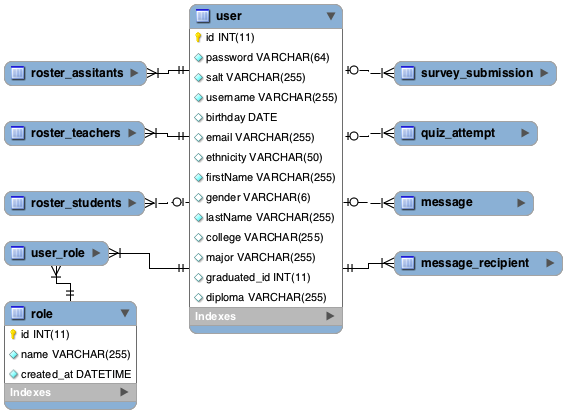
\includegraphics[width=0.7\textwidth]{figures/er/user}
	}
	\caption{User and Role EER Diagram}
	\label{fig:er-user}
\end{figure}

Each of these attributes has an obvious use except, perhaps, for \emph{salt} which is a precautionary security measure. All user passwords are hashed using using the SHA-256 cryptographic hash function. This means that if two users had the same password, then they would obviously result in identical hashes. This fact can be used exploited by people that have large masses of precomputed hashes. A salt, which is a randomly generated string, is append to the plaintext of a password before it is hashed. Now, even if the user's password is something common, what is hashed is, most likely, something unique.

For the sake of simplicity, we decided that the personal/education attributes \emph{birthday}, \emph{email}, \emph{ethnicity}, \emph{gender}, \emph{college}, \emph{major}, \emph{diploma}, and \emph{graduated} as year-independent data. This means that if and when these attributes have a value, that it will not vary based on what academic year the client has selected to be the current year; their values will persist through all years. On the other hand, there is strictly educational data that we do treat as year-dependent: activities, courses, exams, and grade level.

\begin{figure}[h!]
	\centering
	\fbox{
		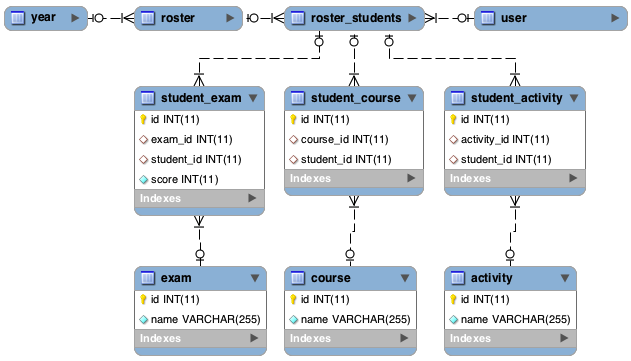
\includegraphics[width=0.7\textwidth]{figures/er/user-student}
	}
	\caption{Student user EER Diagram}
	\label{fig:er-user-student}
\end{figure}

Figure \ref{fig:er-user-student}, outlines the general model to achieve a year-dependent relationship between a student and their educational data and will be explained in depth in \S \ref{subsec:design-district}. Any given year is associated with many rosters, each of which contain a set of students in varying grade levels. Each student in a roster can then be associated with many exams, courses, and activities. 

\subsubsection{Implementation}
User management is broken up into three processes: creation, updating, and reading. As an interface to each of these processes, privileged users have access to a user management interface seen in Figure \ref{fig:screens-user-list}. This interface will only display the users that the currently authenticated user has access to. For administrators, this will be all users, whereas a teacher or a teaching assistant will only see the students that belong to the district that themselves belong to. For example, if a teacher is listed as being a teacher in the district ``Public School \#1'' for the year 2011, then the user list will only show students that also enrolled at the district during that year.

This idea of teachers and teaching assistants only having access to the students that are on the same roster as them is persistent throughout the application. The details regarding districts, rosters, and permissions will be explained in \S \ref{subsec:design-district}.

With this data now being tracked by the Collaborative Environment, trends and reports will be able to be generated. Tracking student participation in activities, courses, and exams is now possible for the set of all students or even subsets such as minorities, males, or females.

\begin{figure}[h!]
	\centering
	\fbox{
		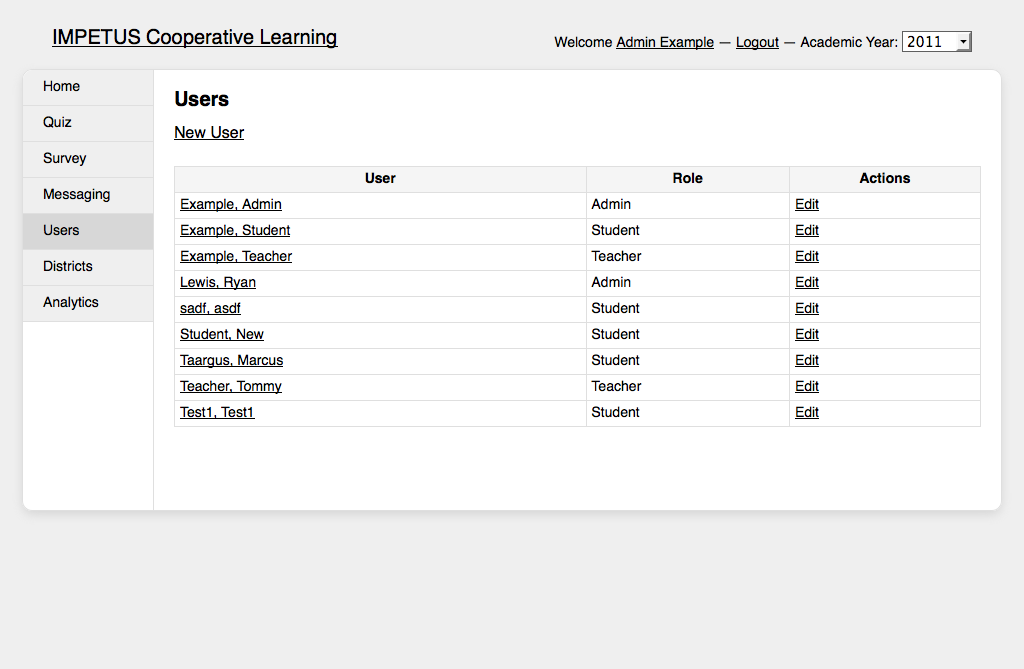
\includegraphics[width=0.8\textwidth]{figures/screens/user/user-list}
	}
	\caption{A privileged user's view of all the system's users.}
	\label{fig:screens-user-list}
\end{figure}

When a privileged user must add or edit a user, the interface appears as it does in Figure \ref{fig:screens-user-student-edit}, except all of the fields are simply blank in the case of adding a new user. The interface has has been split horizontally into two sections, the top is for personal/educational data whereas the bottom is for strictly educational data. In the top half, input fields has been grouped into sets of required and supplemental (optional). This allows the user to readily identify which fields they must have a value for and not have to wait for the program to return an error.

\begin{figure}[h!]
	\centering
	\fbox{
		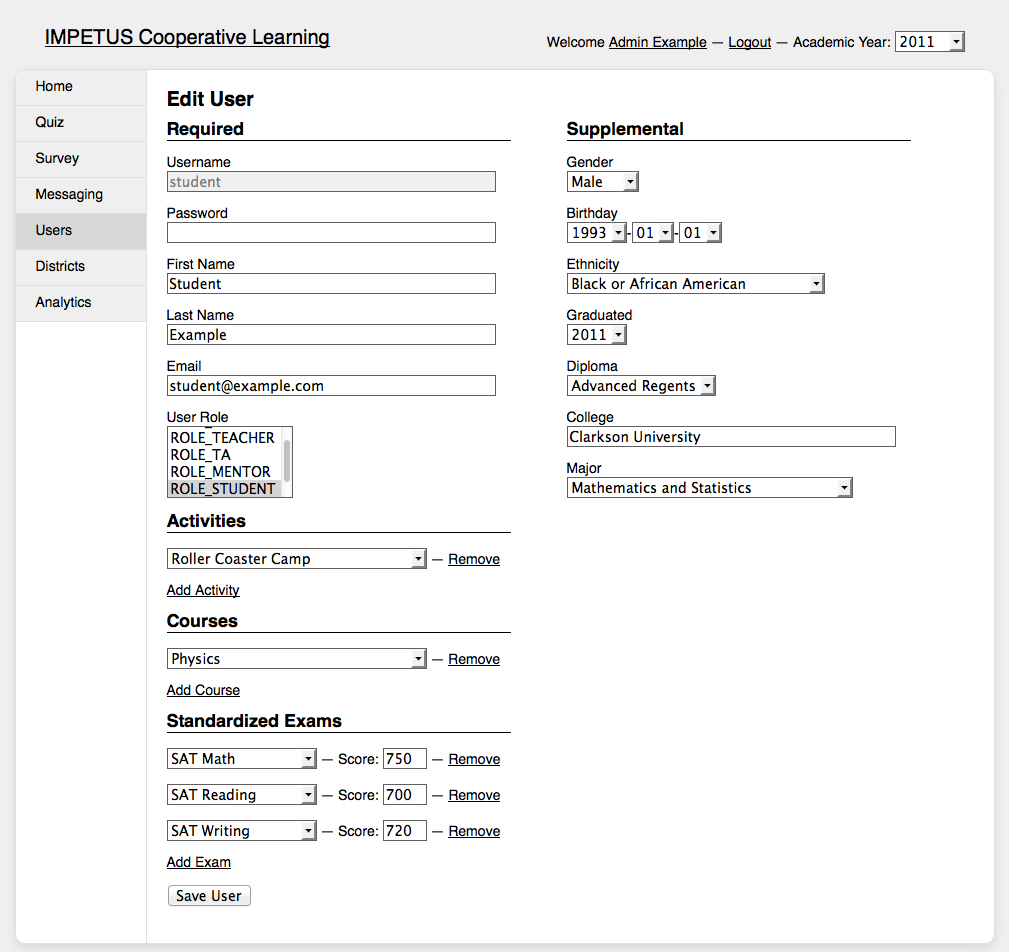
\includegraphics[width=0.8\textwidth]{figures/screens/user/user-student-edit}
	}
	\caption{A privileged user editing a student's account.}
	\label{fig:screens-user-student-edit}
\end{figure}

The supplemental fields for \emph{ethnicity}, \emph{diploma}, and \emph{major}, provide the user with a limited selection of options rather than a freely fillable text input because this will allow for consistent data analysis. If users were able to enter whatever they wanted for these, it would become difficult to use that data to generate accurate reports. For example, if one person were to enter that a student was going to major in ``Mathematics'' and another were to enter ``Math''.

Since the bottom half of the screen only applies to students, where strictly educational data is entered, it will only appear if the user is assigned the Student role. As stated in the Implementation section, \emph{activities}, \emph{courses}, and \emph{exams} are year-dependent. This means that if a user were to choose different academic years while editing a student's data, they would see these fields change appropriately. A student can be associated with as many year-dependent  fields as necessary by clicking the Add button for the appropriate section.

Lastly, viewing user data in a more organized fashion is shown in Figure \ref{fig:screens-user-student-profile}. This simply provides an view into the data stored for a user. Just as the add/edit screen would update its data when the current academic year is changed, so will the view screen.

\begin{figure}[h!]
	\centering
	\fbox{
		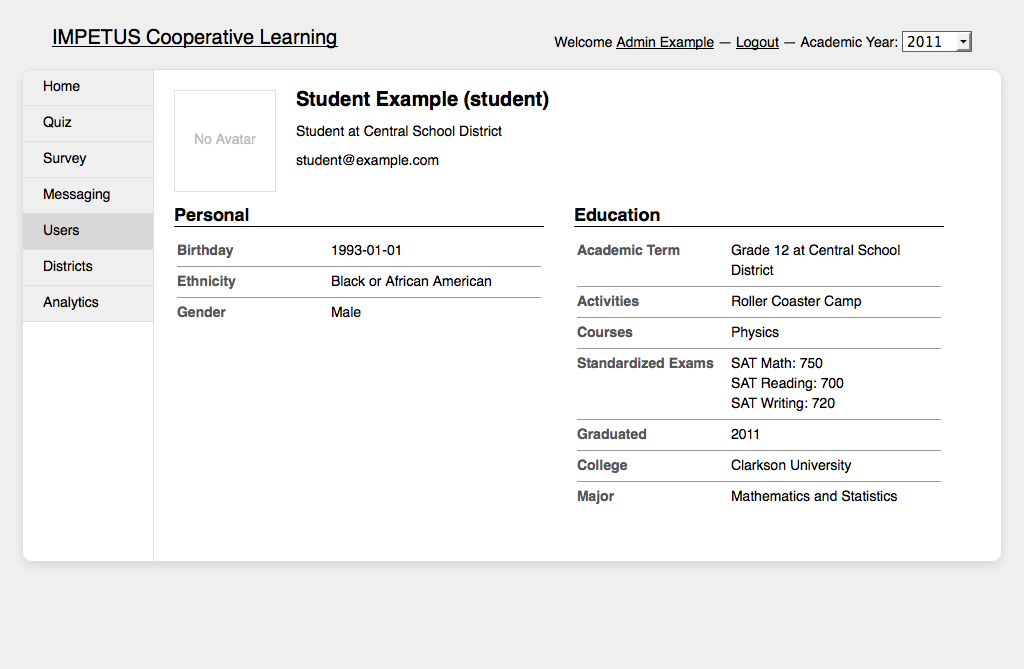
\includegraphics[width=0.8\textwidth]{figures/screens/user/user-student-profile}
	}
	\caption{A privileged user's view of a student's profile.}
	\label{fig:screens-user-student-profile}
\end{figure}


%%%% Districts
\subsection{District Management}
\label{subsec:design-district}
In order to more accurately group the Collaborative Environment's users together and to control access to private student data, a district entity is necessary. If a district was to only ever have the same users associated with it, then a district entity alone would be sufficient, but this is not true; a district's relationship with its teachers, teaching assistants, and students is year-dependent. To allow for this, we introduce the idea of a roster entity where a district can have many rosters such that each roster is associated with a single year.

Using this grouping, it is now also possible to allow access to data based upon which roster a user belongs to. For instance, teachers could be given access to only the students in the roster that they themselves are apart of for a given year, thus they would not be allowed to see student performance in another district. Having a district associated with a student for any given also allows for a wider range of data analysis as it becomes possible to, for instance, compare student performance between districts.

\subsubsection{Design}
Using the concept of a roster, it becomes a join table (a table which links common attributes between two or more tables, in this case \emph{year\_id} and \emph{district\_id}) for the district's  many-to-many relationship with a year. In other words, a district will be associated with many years because it will have a different set of users each year. Likewise, a year will be associated with many districts because each academic year, the Collaborative Environment will be tracking multiple school districts.

\begin{figure}[h!]
	\centering
	\fbox{
		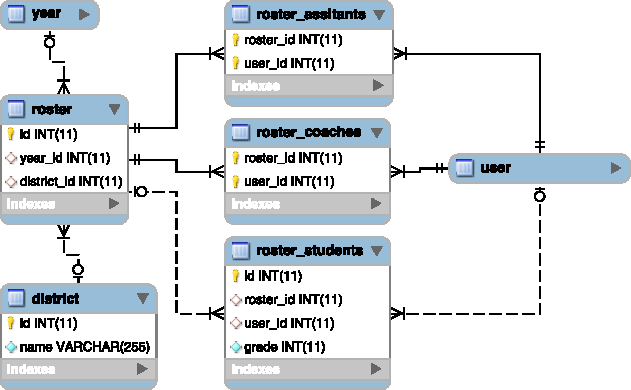
\includegraphics[width=0.7\textwidth]{figures/er/district.pdf}
	}
	\caption{District and Roster EER}
	\label{fig:er-district}
\end{figure}

Figure \ref{fig:er-district} shows the many-to-many relationship between district and year via roster. In addition to being a join table, roster must be uniquely identifiable itself since it must be in a many-to-many relationship with the user table, therefore it has its own \emph{id}. To keep track of a district's three groups of users for a given year (teaches, teaching assistants, and students), its roster maintains three different relationships with the user table. If a user is a teacher and is to be in a district's roster for a given year, then they will be added to the roster\_teacher table. The same logic applies to assistants and students, except a student can additionally have a \emph{grade} associated with them (e.g. grade 9, grade 10).

\subsubsection{Implementation}
Privileged users have access to the a list of the districts, as show in Figure \ref{fig:screens-district-list}, which they are in the rosters of for the currently selected year where they can a. An exception to this is for administrators, which have access to all districts. From this list, privileged users can edit any district in the list and administrators have the additional ability to create a new district.

\begin{figure}[h!]
	\centering
	\fbox{
		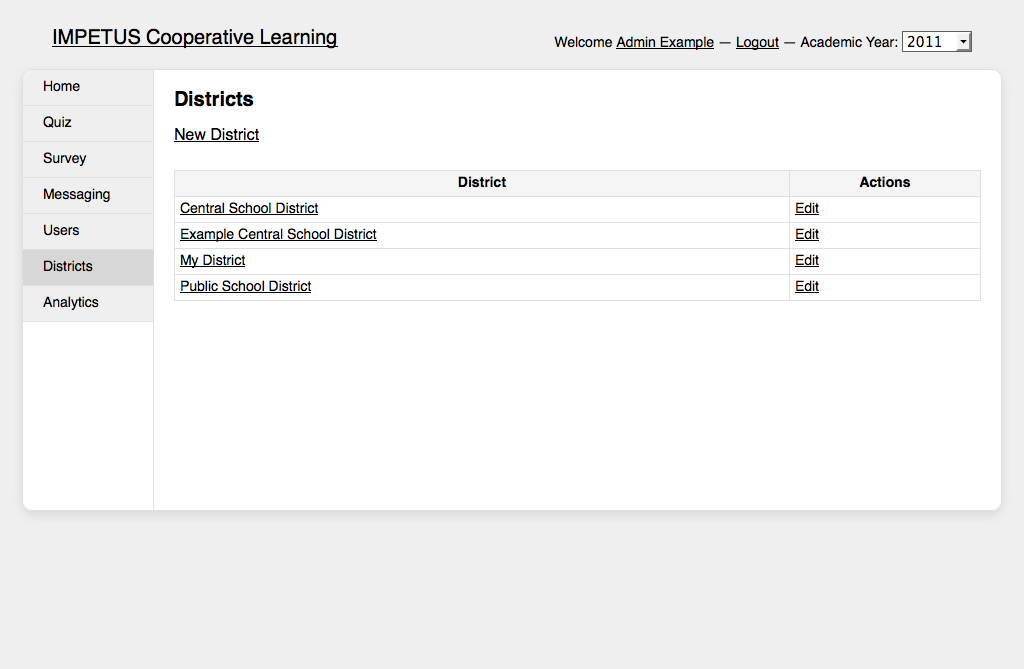
\includegraphics[width=0.8\textwidth]{figures/screens/district/district-list}
	}
	\caption{An administrator's view of all the system's districts.}
	\label{fig:screens-district-list}
\end{figure}

When editing or adding a district, the user will use the interface displayed in Figure \ref{fig:screens-district-edit}. One is able to add users of different classes to the roster by searching for their name in the appropriate search boxes. In this initial implementation, there is a constraint such that teachers and students can only be in one district's roster for a given year. This was set because, in most cases, teachers and students generally do not need to be associated with multiple districts. Due to this limitation, users that are already in a different roster for the current year will not appear in the search results for a user.

\begin{figure}[h!]
	\centering
	\fbox{
		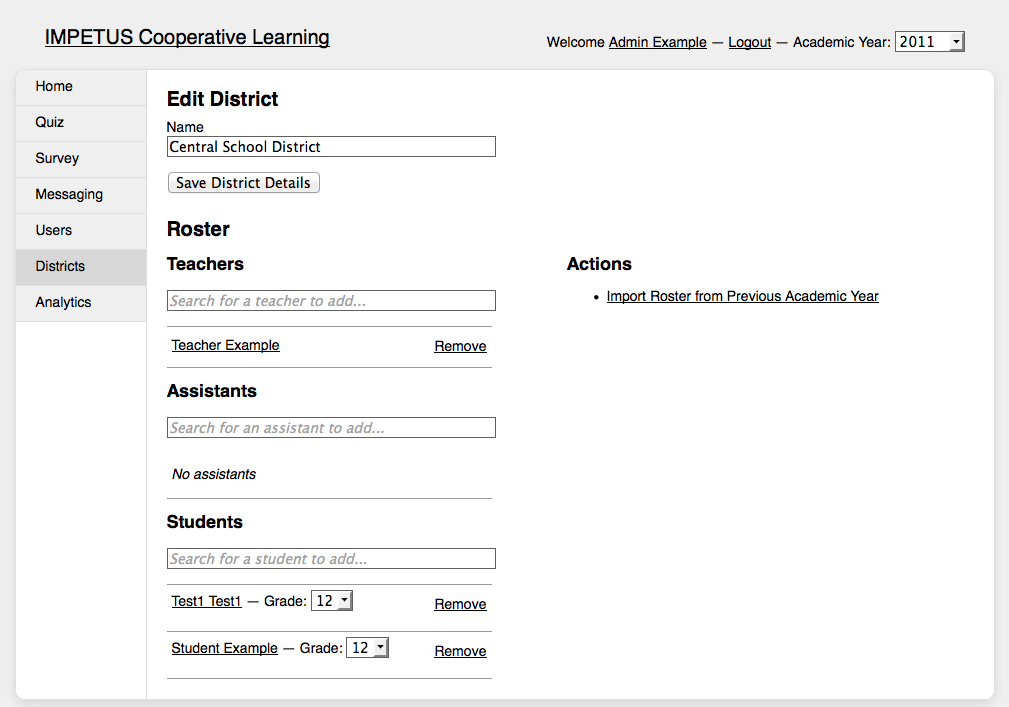
\includegraphics[width=0.8\textwidth]{figures/screens/district/district-edit}
	}
	\caption{A privileged user editing a district.}
	\label{fig:screens-district-edit}
\end{figure}

Each new academic year, a roster will need to be created that ties the districts to that new year. This can be a tiresome activity, especially if a district has a lot of users that need to be associated with it. To try to ease this process, there is an import feature which will simply look at the previous year's roster for the current district and copy it to the current year's roster. It will also automatically increment the student's grades by one; this is due to the assumption that a majority of students will advance to the next grade.

\subsection{Learning Pathway}
\label{subsec:design-pathway}
test

\subsubsection{Design}
test

\subsubsection{Implementation}
test

%%%% Quiz
\subsection{Quiz System}
\label{subsec:design-quiz}
A system by which teachers and teaching assistants can create assessments of their student's knowledge is one of the key collaborative goals of this system. By allowing teachers and teaching assistants to create quizzes quickly and easily, it will allow them to get valuable feedback from their students. From the student's perspective, they'll have access to a means of studying and brushing up on topics that they might feel they are struggling with. A quiz can be made about any topic, but when used in conjunction with the learning pathway, as described in \S \ref{subsec:design-pathway}, it creates a rich means of showing students the topics they need to know (based on state standards) while providing them with the resources to succeed.

\subsubsection{Design}
A quiz in the Collaborative Environment can be broken up into two sets of relationships: a quiz, its questions, and its questions answers and a student, their attempt at a quiz, and how they performed on each question during that attempt. Figure \ref{fig:er-quiz} shows that one quiz may have multiple questions and that a question may have multiple answers. This approach allows for two different types of questions to be used in a quiz: short answer and multiple choice. If a quiz question only has one answer, then it is a short answer, whereas if it has multiple answers then it is clearly a multiple choice question.

\begin{figure}[h!]
	\centering
	\fbox{
		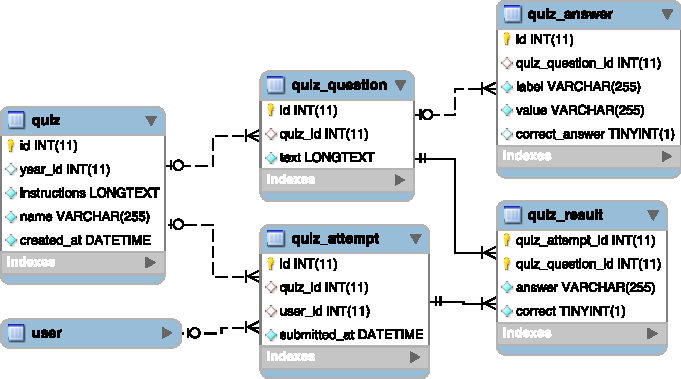
\includegraphics[width=0.7\textwidth]{figures/er/quiz.pdf}
	}
	\caption{Quiz and Quiz Result EER}
	\label{fig:er-quiz}
\end{figure}

To allow students the ability to learn from their mistakes, quizzes may have multiple attempts made at them to achieve a perfect score. This requires that a user have a many-to-many relationship with a quiz itself via an attempts join table. To be able to store exactly which questions a student got correct or incorrect along with their actual answer, every quiz attempt has a many-to-many relationship with a quiz's questions called result. The idea is that an individual attempt at a quiz is comprised of a series of results, or a result of answering each quiz question. Each result is able to store the exact answer that a student gave along with if it was correct.

\subsubsection{Implementation}
When a privileged user wants to create a quiz, they will be presented with the interface seen in Figure \ref{fig:screens-quiz-new}. First, the creator must choose a name for the quiz and may enter instructions for the student to follow. Next, the creator may add as many problems to the quiz as they must, each of which they may add one or more answers to.

\begin{figure}[p!]
	\centering
	\fbox{
		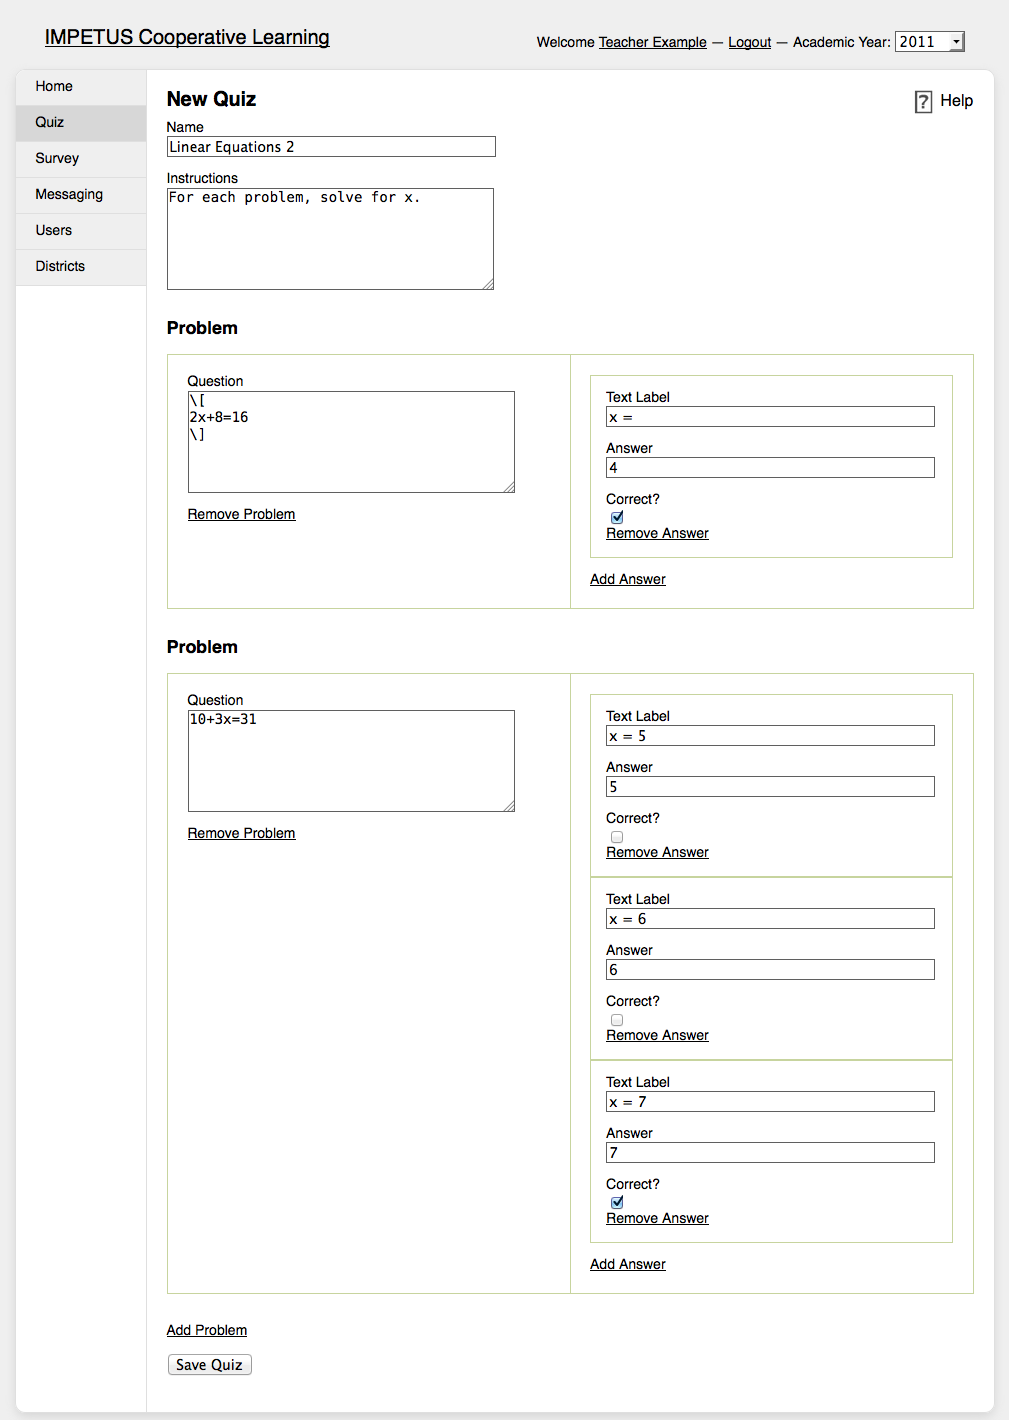
\includegraphics[width=0.8\textwidth]{figures/screens/quiz/quiz-new}
	}
	\caption{A privileged user creating a quiz.}
	\label{fig:screens-quiz-new}
\end{figure}

When adding the text for the question, the creator may opt to use the \LaTeX\ displayed math shorthand (i.e. \texttt{\textbackslash [ ...\textbackslash ]} ). Should they choose to, then their question will be rendered by a JavaScript library called MathJax that displays equations in \LaTeX\ markup in all web browsers. \cite{mathjax-webpage}. If they choose not to, then whatever is entered will simply appear as the question. An example of each can be seen in the questions in Figure \ref{fig:screens-quiz-new}.

As stated in the design section, a question can have one or more answers associated with it. If it has only one answer, it makes it a short answer question allowing the student and freely type in an answer. The creator must include a ``text label'' for the answer which is what will appear before the text input when attempting the quiz (e.x. ``$x = $''). If the question has multiple answers (making it a multiple choice question), then this same text label becomes the visible text identifying one answer from another.

Switching to the perspective of a logged in student, they would see the interface show in Figure \ref{fig:screens-quiz-list-student} which displays the available quizzes, some of which the student has attempted and one of which that they have not.

\begin{figure}[h!]
	\centering
	\fbox{
		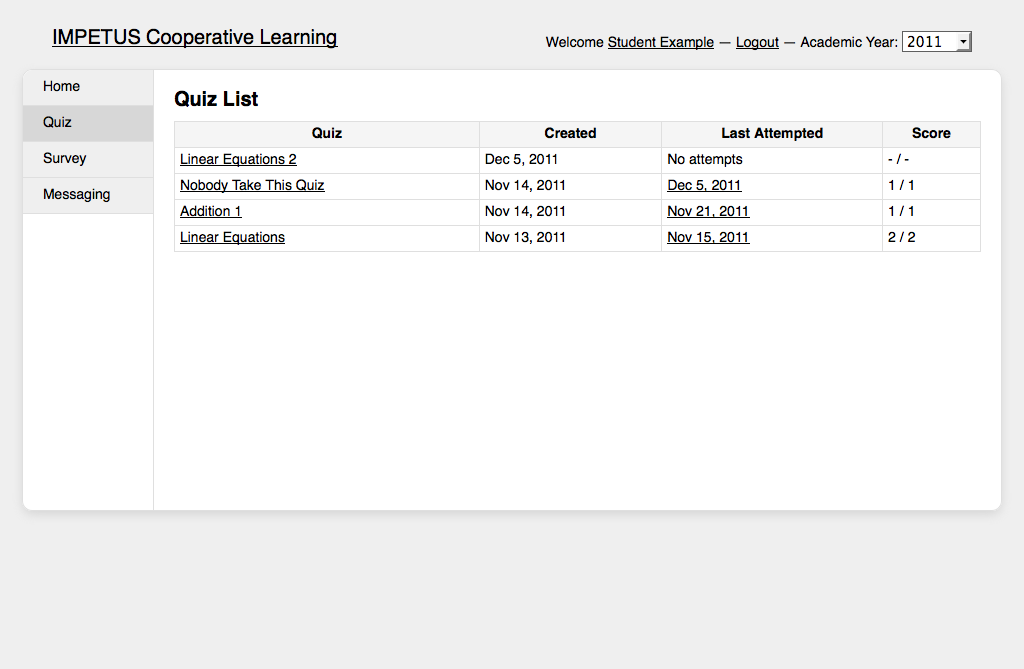
\includegraphics[width=0.8\textwidth]{figures/screens/quiz/quiz-list-student}
	}
	\caption{A student's list of available quizzes.}
	\label{fig:screens-quiz-list-student}
\end{figure}

If the student were to attempt the ``Linear Equations 2'' quiz, they would then they would be presented with what is shown in Figure \ref{fig:screens-quiz-new-attempt}; a rendered version of what was being constructed in Figure \ref{fig:screens-quiz-new}. One can see that ``Problem 1'' has a styling that looks identical to what one would expect to see in \LaTeX\ rendered document as well as a plaintext question in ``Problem 2''. ``Problem 1'' is a demonstration of a short answer question and allows the user to freely type in an answer whereas ``Problem 2'' is clearly a multiple choice question.

\begin{figure}[h!]
	\centering
	\fbox{
		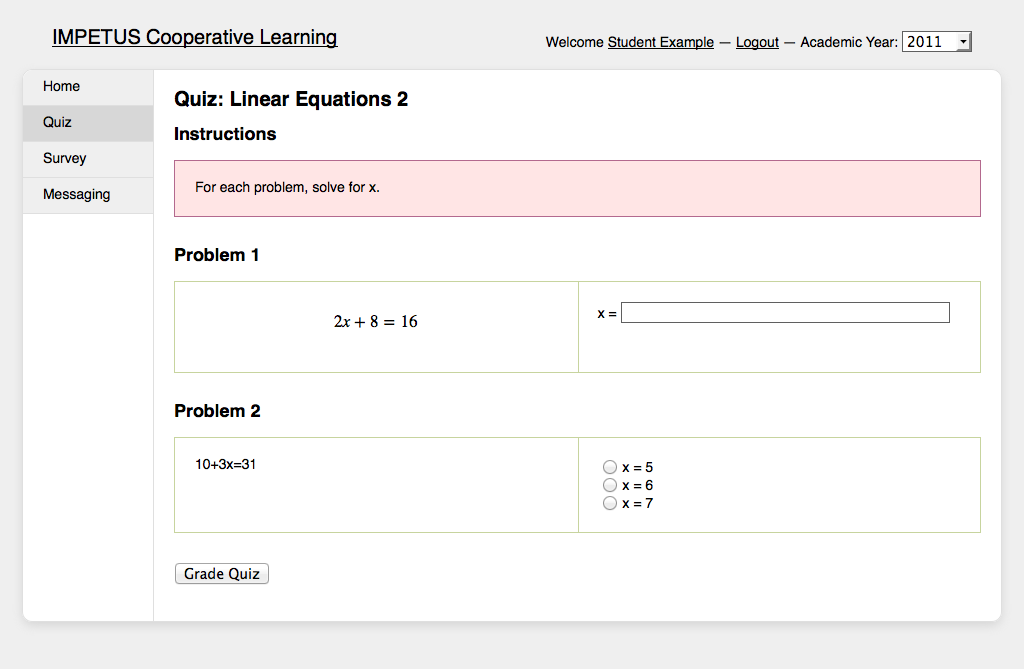
\includegraphics[width=0.8\textwidth]{figures/screens/quiz/quiz-new-attempt}
	}
	\caption{A student attempts a new quiz.}
	\label{fig:screens-quiz-new-attempt}
\end{figure}

When a student enters their answers for the quiz, the system will simply compare their answers to answers that were set during quiz creation. This implementation can only exactly compare a student's input to the values that were given during a quiz's creation (e.g. it can not round or reduce answers). The results of submitting a quiz for grading can be seen in Figure \ref{fig:screens-quiz-attempt-results}.

\begin{figure}[h!]
	\centering
	\fbox{
		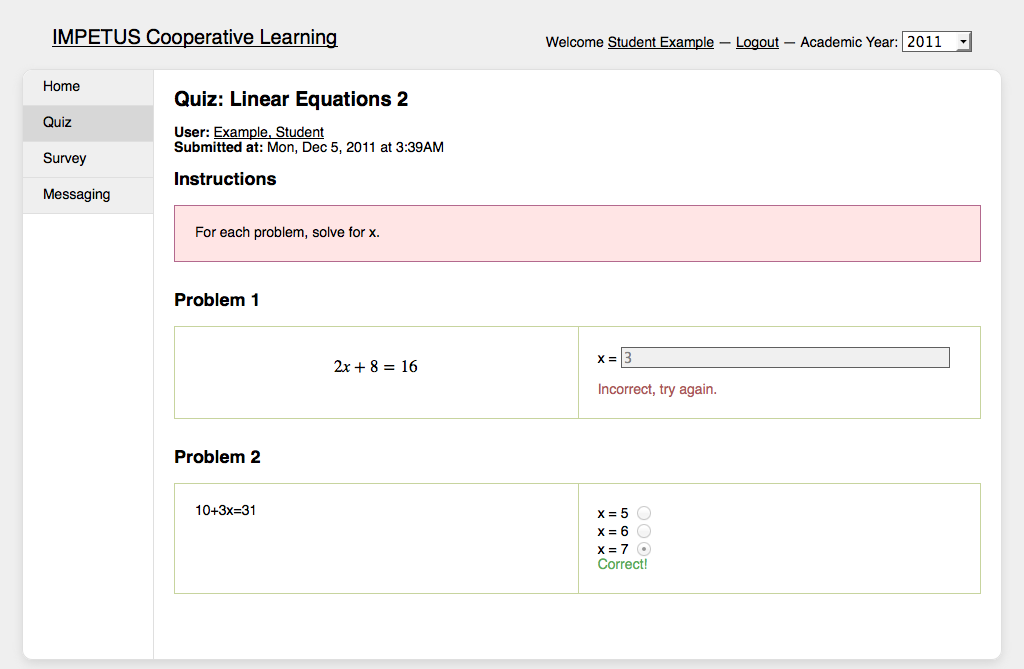
\includegraphics[width=0.8\textwidth]{figures/screens/quiz/quiz-attempt-results}
	}
	\caption{A student receives the results of their quiz attempt.}
	\label{fig:screens-quiz-attempt-results}
\end{figure}

As previously stated, students have the option of taking a quiz as many times as they see fit and the system will, in turn, keep track of those attempts. This allows for analyzing student performance on individual topics and for assessing the quality of quizzes. We see the list of attempts that was made on the ``Linear Equations 2'' quiz in Figure \ref{fig:screens-quiz-attempt-list}.

\begin{figure}[h!]
	\centering
	\fbox{
		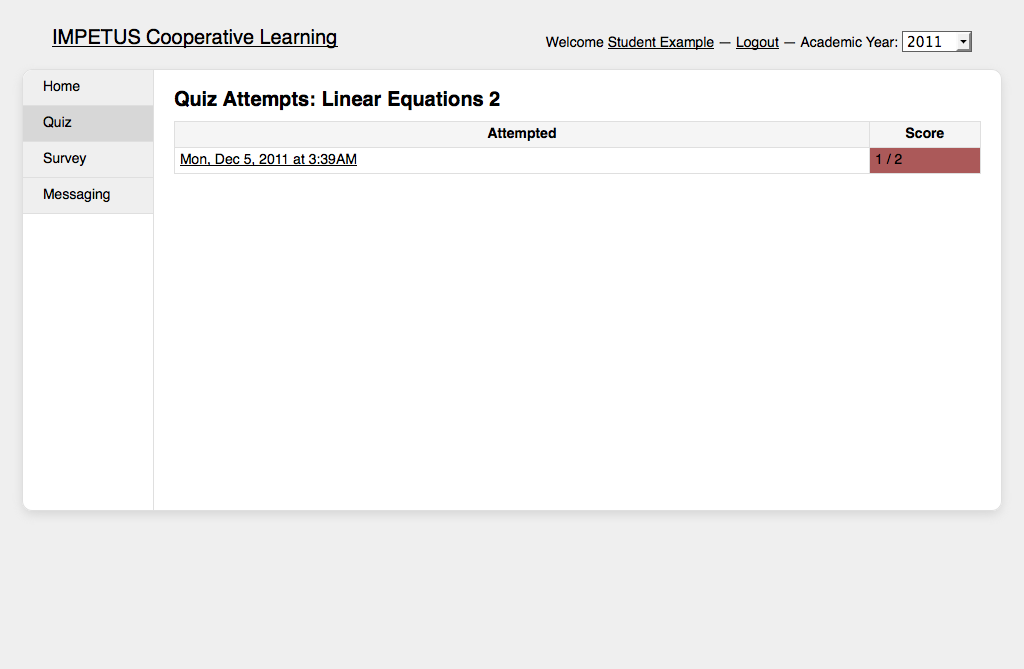
\includegraphics[width=0.8\textwidth]{figures/screens/quiz/quiz-attempt-list}
	}
	\caption{A student views all of their attempts at a quiz.}
	\label{fig:screens-quiz-attempt-list}
\end{figure}

Once students start answering quizzes, teachers and teaching assistants are able to see their progress on them from the results interface show in Figure \ref{fig:screens-quiz-results-list}. The viewing policy on quiz results is that teachers and teaching assistants may only see the students that are in the same district roster as them for the currently selected year (see \S \ref{subsec:design-district} for details of the district and roster design).

\begin{figure}[h!]
	\centering
	\fbox{
		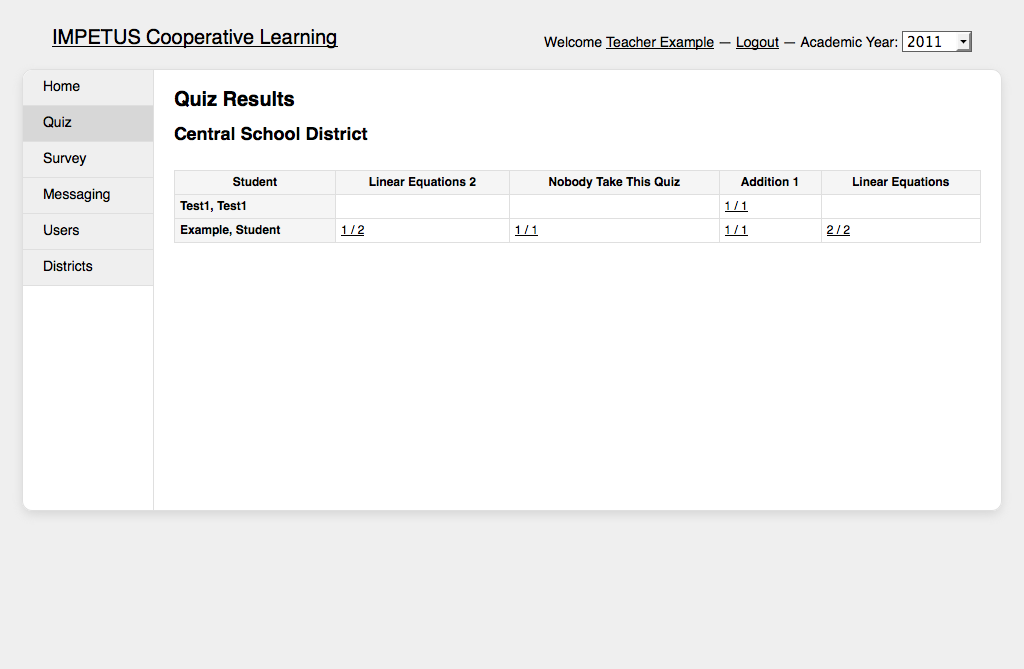
\includegraphics[width=0.8\textwidth]{figures/screens/quiz/quiz-results-list}
	}
	\caption{A teacher views the quiz results of the students in their district.}
	\label{fig:screens-quiz-results-list}
\end{figure}

%%%% Survey
\subsection{Survey System}
\label{subsec:design-survey}
test

\subsubsection{Design}
test

\begin{figure}[h!]
	\centering
	\fbox{
		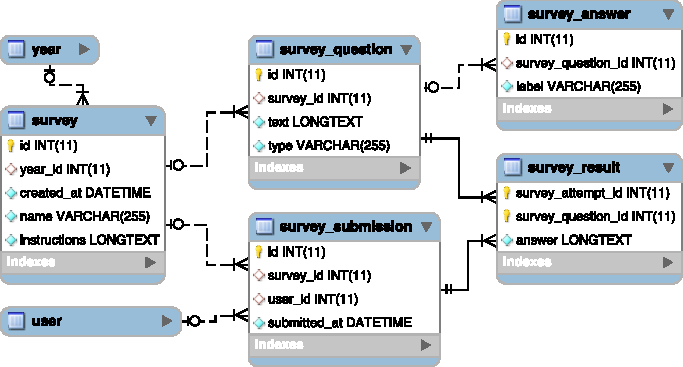
\includegraphics[width=0.7\textwidth]{figures/er/survey.pdf}
	}
	\caption{Survey and Survey Submission EER}
	\label{fig:er-survey}
\end{figure}

\subsubsection{Implementation}
test

%%%% Messaging
\subsection{Messaging}
\label{subsec:design-messaging}
To facilitate communication between all of these users, a messaging system was devised that would allow for a quick means of contacting either a user or a group of users. A problem that IMPETUS has continuously faced is that of organizing the contact information of all its associated people. There was no quick way to contact students and contacting teachers involved sorting through contact lists.

As a solution to this, the Collaborative Environment has a simple messaging system that allows for contacting any of the systems registered users. One may send a message to just an individual, a group of individuals, or even an entire class of users quickly. The system keeps track of messages internally, but is capable of notifying a user of a new message via email if they have an email address associated with their account.

\subsubsection{Design}
The messaging system treats messages and their replies as a correspondence thread, that is, one message is a parent and then replies may be added after that parent. When a new message is created, a single instance of that message is stored in the message table (see Figure \ref{fig:er-message}). All of the designated recipients are then added to the recipient table, including the sender themselves. This means that even though a message will be sent to at least two people, there is only ever one instance of the message itself and all recipients are basically given viewing rights to that message via the recipients table. When a user has opened a message or deletes it, their entry in the recipients table for that message is simply modified.

If a message is a reply to a parent, then its entry in the message table is marked as such and all the recipients of the parent message will then receive a copy of the reply.

Having a message system built like this allows for an archive of messages and reduces message text duplication in the database.

\begin{figure}[h!]
	\centering
	\fbox{
		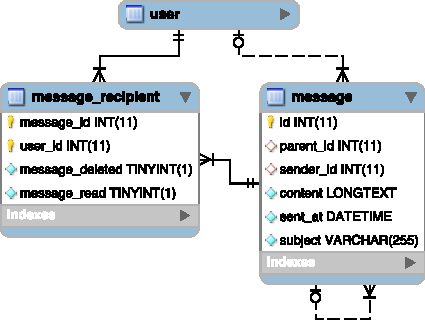
\includegraphics[width=0.4\textwidth]{figures/er/message.pdf}
	}
	\caption{Message and Message Recipient EER}
	\label{fig:er-message}
\end{figure}

\subsubsection{Implementation}
As stated previously, any registered user in the system has access to the messaging feature and, as such, can message any other user in the system. In Figure \ref{fig:screens-message-new}, a student is sending their teacher a message regarding a homework assignment. The ``To'' field allows for any number of recipients to be added to it via an autocompleting search feature. Recipients can also be classes of users such as ``Students'' as a quick way of addressing all the users in the system that have the student role. Upon sending the message, it will appear in both the sender's and the recipient's message lists (but in the case of the sender, it will be marked as read). Additionally, if the recipients have an email address associated with their account, a copy of the message will be sent to that address along with a link to view the message in the Collaborate Environment. The message list acts as a combination of an inbox and an outbox.

\begin{figure}[h!]
	\centering
	\fbox{
		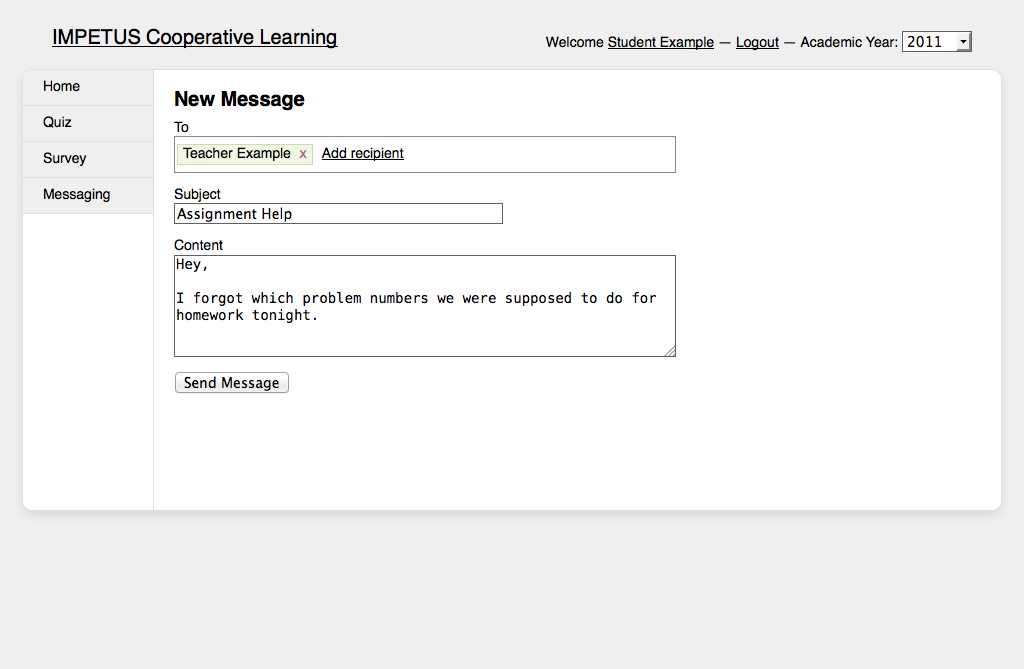
\includegraphics[width=0.8\textwidth]{figures/screens/message/message-new}
	}
	\caption{A student sends a new message to their teacher.}
	\label{fig:screens-message-new}
\end{figure}

When the teacher that was marked as the recipient of the student's message checks their message list (Figure \ref{fig:screens-message-list}), they will see it at the top and highlighted as it is an unread message.

\begin{figure}[h!]
	\centering
	\fbox{
		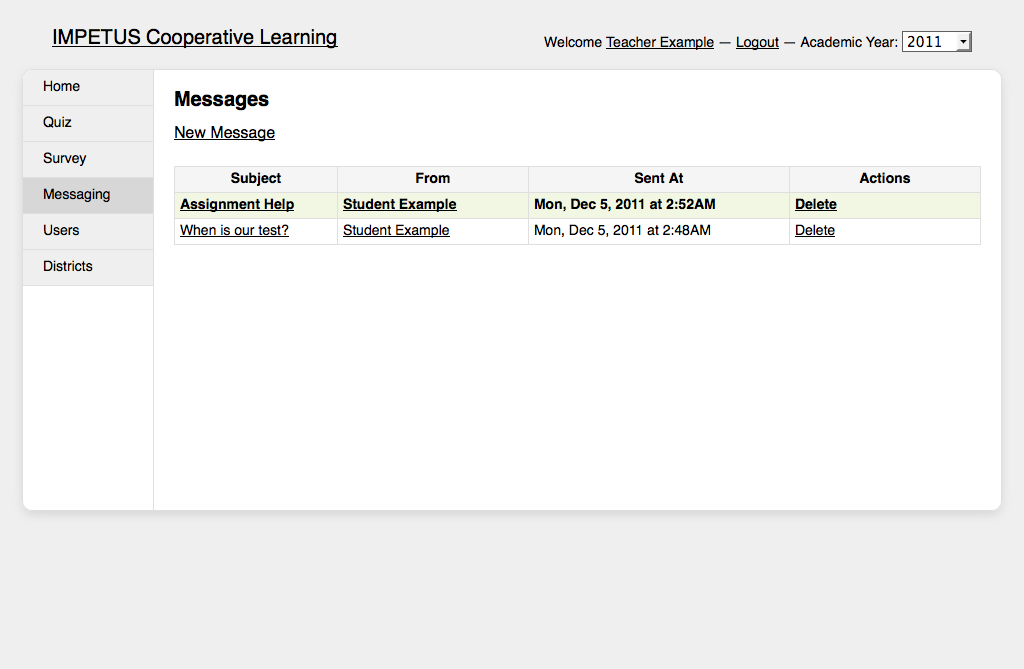
\includegraphics[width=0.8\textwidth]{figures/screens/message/message-list}
	}
	\caption{A teacher views their message list.}
	\label{fig:screens-message-list}
\end{figure}

Viewing a message will open the chain of messages with the parent at the top. In this case, since the student was the original sender, their message will appear at the top of the list and replies will be appended. The teacher responds the student's inquiry, as shown in Figure \ref{fig:screens-message-reply}, and an email will be sent to the student, if appropriate, notifying them of the response. If the teacher were to return to their message list, the thread of messages will now be marked as unread.

\begin{figure}[h!]
	\centering
	\fbox{
		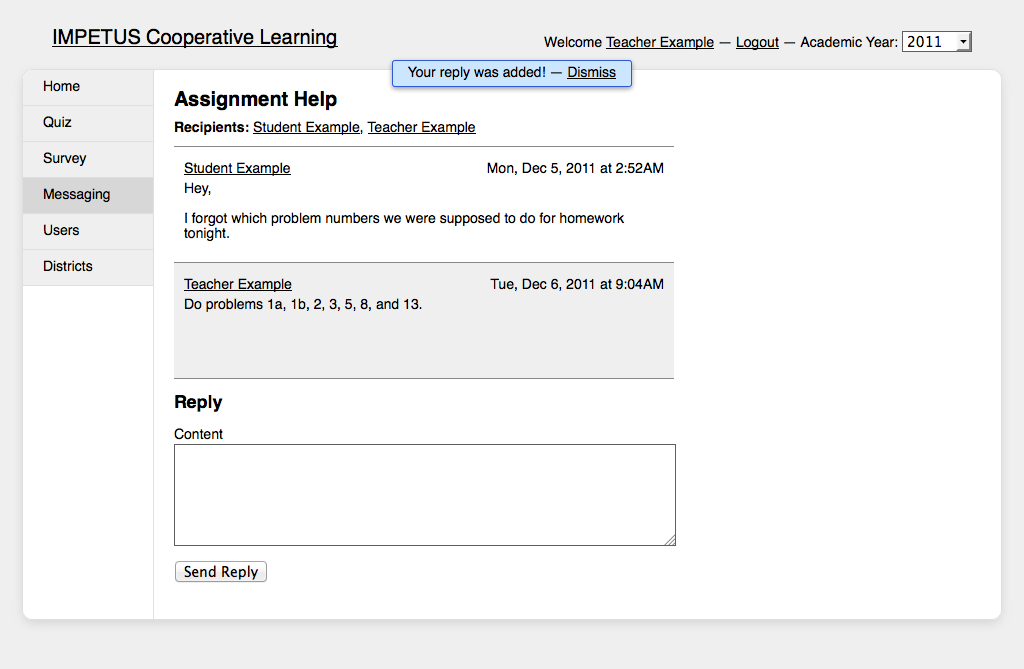
\includegraphics[width=0.8\textwidth]{figures/screens/message/message-reply}
	}
	\caption{A teacher replies to a student's message.}
	\label{fig:screens-message-reply}
\end{figure}

%%%% Analytics
\subsection{Analytics}
\label{subsec:design-analytics}
test

\section{Known Issues}